\documentclass{article}
\usepackage{amsmath,amssymb}
\usepackage{fullpage}
\usepackage{mathrsfs}
\usepackage{setspace}
\usepackage{graphicx}
\usepackage{listings}
\usepackage{multirow}
\renewcommand{\baselinestretch}{1}
\pagestyle{empty}
\usepackage{color}
\definecolor{dkgreen}{rgb}{0,0.6,0}
\definecolor{gray}{rgb}{0.5,0.5,0.5}
\definecolor{mauve}{rgb}{0.58,0,0.82}

\lstset{frame=tb,
	language=Matlab,
	aboveskip=3mm,
	belowskip=3mm,
	showstringspaces=false,
	columns=flexible,
	basicstyle={\small\ttfamily},
	numbers=none,
	numberstyle=\tiny\color{gray},
	keywordstyle=\color{blue},
	commentstyle=\color{dkgreen},
	stringstyle=\color{mauve},
	breaklines=true,
	breakatwhitespace=true,
	tabsize=4
}
\usepackage{tikz}
\begin{document}
\noindent{\bf Homework 8}

\noindent{\bf Jingmin Sun}

\noindent{\bf 661849071}

\begin{enumerate}
\item
\begin{enumerate}
\item
\begin{align*}
I&=\int_1^4 \ln (x) dx\\
&= x \ln x| _{x=1}^4 - \int_{x=1}^4 x d\ln(x)\\
&= x \ln x |_{x=1}^4 -\int_{x=1}^4 x \dfrac{1}{x} dx\\
&=4\ln 4-\ln 1 -(4-1)\\
&=4\ln 4 -3
\end{align*}
\item

 \lstinputlisting[language=Matlab, numbers=left, stepnumber=1, firstline=1, frame = single,caption={two\_point\_Gaussian.m}]{two_point_Gaussian.m}
 
 and the output table is \begin{small}
 \lstinputlisting[language=Matlab,caption={output}]{two_point_output.txt}
 \end{small}
 
 \item
 
  \lstinputlisting[language=Matlab, numbers=left, stepnumber=1, firstline=1, frame = single,caption={three\_point\_Gaussian.m}]{three_point_Gaussian.m}
 
 and the output table is \begin{small}
 \lstinputlisting[language=Matlab,caption={output}]{three_point_output.txt}
 \end{small}
 \item
From the above analysis, we found that when we increase the number of mesh, which decrease the interval of each mesh at the same time, increases the accuracy of the approximation, and when we use more point on a mesh, we will get a more accurate approximation as well. To see this more clearly, we can draw the graph of error term:  \begin{center}
  \includegraphics[width=6cm]{error_analysis_Gaussian.jpg} 
 \end{center}
 
 Beside that, we can see that the three point Gaussian will converge faster, which means generating an error of higher order. To get the numerical order, we can compute the base 2 log of reduction factor of each method, which is the slope of two plotted lines (without negative sign):\begin{small}
 \lstinputlisting[language=Matlab,caption={error}]{Gaussian_error.txt}
 \end{small}
 So, we can see that this example perform an error greater than third order when $n=1$ (2-point), and greater than fifth order when $n=2$ (3-point). This is related to the d.o.p of these two method, which is  $2n+1$, and this example performs better on both of methods than expected.
\end{enumerate}


\item
\begin{align*}
y_{j+1}&=y_j+h\left(\theta f(t_j,y_j)+(1-\theta) f(t_{j+1},y_{j+1})\right)\\
&=y_j+h\theta f(t_j,y_j)+h(1-\theta) f(t_{j+1},y_{j+1})\\
&=y_j+h\theta f(t_j,y_j)+hf(t_{j+1},y_{j+1})-h\theta f(t_{j+1},y_{j+1})\\
&=y_j+h\theta ry_j+hry_{j+1}-h\theta ry_{j+1}\\
&=(1+h\theta r)y_j +(hr-hr\theta) y_{j+1}\\
(1+hr\theta-hr) y_{j+1}&=(1+h\theta r)y_j\\
y_{j+1}&=\dfrac{1+hr\theta}{1+hr\theta-hr}y_j\\
\therefore Q(rh,\theta)&= \dfrac{1+rh\theta}{1+rh\theta-rh}
\end{align*} \begin{align*}
\left|\dfrac{1+rh\theta}{1+rh\theta-rh}\right| &\leq 1\\
-1\leq \dfrac{1+rh\theta}{1+rh\theta-rh}&\leq 1\\
-1\leq 1 +\dfrac{rh}{1+rh\theta-rh}&\leq 1\\
-2\leq \dfrac{rh}{1+rh\theta-rh}&\leq 0\\
\begin{cases}
1+rh\theta-rh &\geq 0\\
\dfrac{-2}{rh}\geq \dfrac{1}{1+rh\theta-rh}
\end{cases}\\
\end{align*}
From the first equation above we can get $-(1+rh\theta-rh)<1+ rh\theta \leq 1+rh\theta-rh$, which lead the same equation of the second equation above, and from the second equation above, we can get $\dfrac{rh}{-2}\leq 1+rh\theta-rh$, $rh\geq -2-2rh\theta+2rh$, $rh(1-2\theta)\leq 2$, 

\begin{itemize}
\item $\theta \in [0,0.5):$
\begin{align*}
\because 1-2\theta&>0\\
rh&\leq \dfrac{2}{1-2\theta}\\
h&\geq \dfrac{2}{r(1-2\theta)}\\
\because r < 0,& 1-2\theta>0\\
\therefore \dfrac{2}{r(1-2\theta)}&<0\\
\text{Together with } h&>0\\
\therefore h&> 0\\
\end{align*}
\item $\theta=0.5$
\begin{align*}
h \text{ unbounded}\\ \text{Together with } h&> 0\\
\therefore h&>0\\
\end{align*}
\item
$\theta \in (0.5,1]$
\begin{align*}
\because r < 0,& 1-2\theta <0\\
\therefore h&\leq \dfrac{2}{r(1-2\theta)}\\
\dfrac{2}{r(1-2\theta)}&\geq 0\\
\therefore 0< h&\leq \dfrac{2}{r(1-2\theta)}
\end{align*}
\end{itemize}

In conclusion, when $\theta \in [0,0.5]$, $h> 0$, and when $\theta \in (0.5,1]$, $0< h\leq \dfrac{2}{r(1-2\theta)}$
\item
\begin{enumerate}
\item
\begin{align*}
y'&= 2(t+1)y\\
\dfrac{dy}{dt} &= 2(t+1)y\\
\dfrac{dy}{y}&= 2(t+1)dt\\
\int \dfrac{dy}{y}&=\int 2(t+1)dt\\
\ln (y) &= t^2+2t+c\\
\because y(0)&=1\\
\ln(1) &= 0+0+c\\
c&=0\\
\therefore \ln (y) &= t^2+2t\\
y&=e^{t^2+2t}
\end{align*}

\begin{align*}
\dfrac{dy}{dt}&=\dfrac{1}{y^2}\\
y^2 dy&=dt\\
\int y^2 dy &=\int dt\\
\dfrac{y^3}{3}&=t+c\\
\because y(0)&=1\\
\dfrac{1}{3}&=0+c\\
c&=\dfrac{1}{3}\\
\therefore \dfrac{y^3}{3}&=t+\dfrac{1}{3}\\
y^3&=3t+1\\
y&=\sqrt[3]{3t+1}
\end{align*}
\item

In this function, we just create three vectors and update its value in each iteration of a loop, and the code is:
 \lstinputlisting[language=Matlab, numbers=left, stepnumber=1, firstline=1, frame = single,caption={FE1.m}]{FE1.m}
 and we can get the table\begin{small}
 \lstinputlisting[language=Matlab,caption={output}]{FEtable.txt}
 \end{small}
 where T1 is the table of $y' = 2(t+1)y$, and T2 is the table of $y'=\frac{1}{y^2}$
 \item
 
 To draw the graph, we can just separate it into two graph, one for each function, and add a loop to the previously code with different h.
 \lstinputlisting[language=Matlab, numbers=left, stepnumber=1, firstline=1, frame = single,caption={FE2.m}]{FE2.m}
  The graph of the first equation on the left, and that of the second equation on the right: \begin{center}
  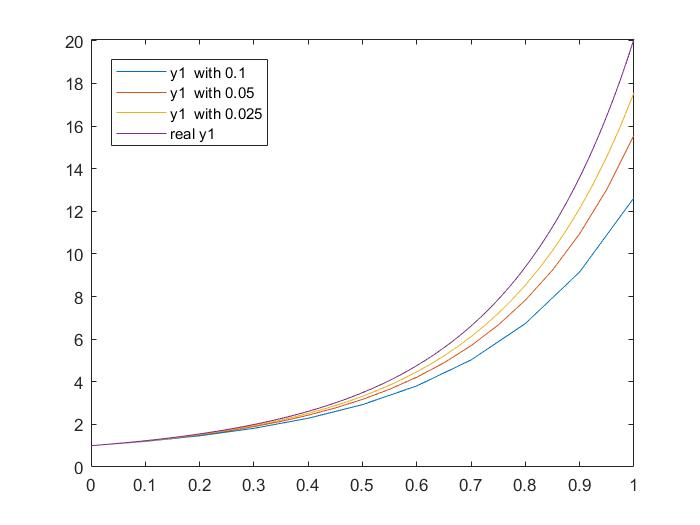
\includegraphics[width=7cm]{y1.jpg} 
    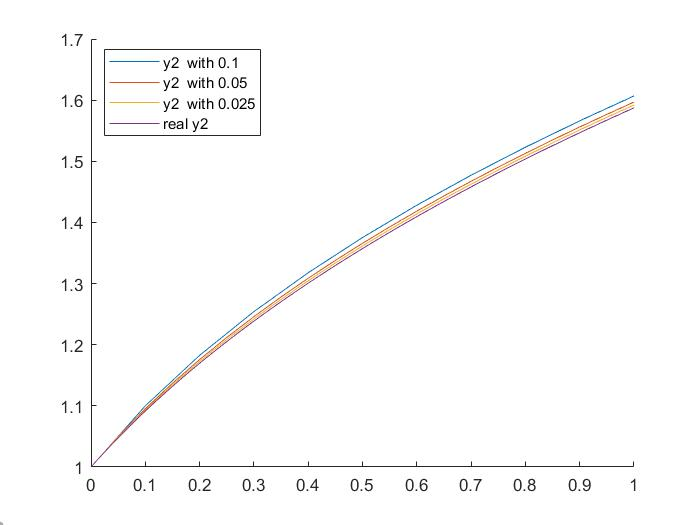
\includegraphics[width=7cm]{y2.jpg} 
 \end{center}

 \item

To plot the error of the function value at $t=1$, we just need to update each y in ecey iteration, instead of store it, and the code is: 
 \lstinputlisting[language=Matlab, numbers=left, stepnumber=1, firstline=1, frame = single,caption={FE3\_loglog.m}]{FE3_loglog.m}
 and we can see the graph:
 \begin{center}
  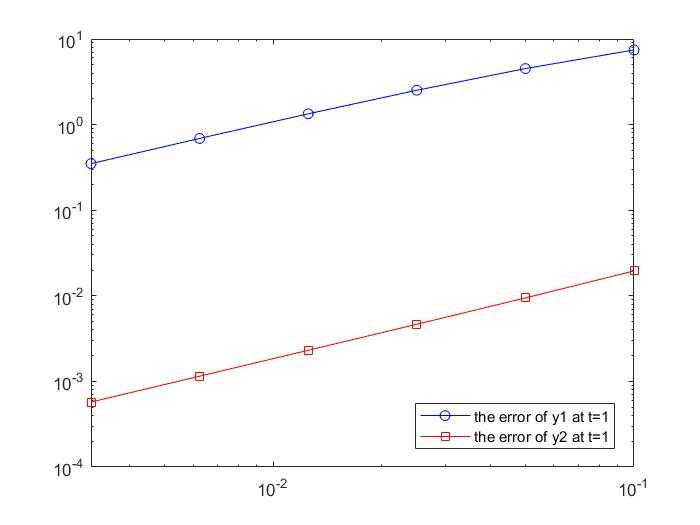
\includegraphics[width=7cm]{FE_loglog.jpg}  
 \end{center}
 We can observe that they have the same slope, and this is consistence with that FE has convergence scheme of order 1.
 \item
 Since for trapzoid method, we have \begin{align*}
 y_{j+1}&=y_j + h (\dfrac{1}{2} f(t_j,y_j)+\dfrac{1}{2}f(t_{j+1}, y_{j+1}))\\
y_{j+1}-\dfrac{h}{2}f(t_{j+1}, y_{j+1})&=y_j+\dfrac{h}{2}f(t_j,y_j)
 \end{align*}
 So for the first equation: \begin{align*}
 y_{j+1}-\dfrac{h}{2} (2(t_{j+1}+1)y_{j+1})&=y_j+\dfrac{h}{2}(2(t_{j}+1)y_{j})\\
  y_{j+1}-h (t_{j+1}+1)y_{j+1}&=y_j+h(t_{j}+1)y_{j}\\
  y_{j+1}&=\dfrac{1+h(t_{j}+1)}{1-h (t_{j+1}+1)}y_j
 \end{align*}
  So for the second equation: \begin{align*}
 y_{j+1}-\dfrac{h}{2} (\frac{1}{y_{j+1}^2})&=y_j+\dfrac{h}{2}(\frac{1}{y_j^2})\\
 \dfrac{2y_{j+1}^3-h}{2y_{j+1}^2}&=\dfrac{2y_{j}^3+h}{2y_{j}^2}
 \end{align*}
 And for this one, we can use matlab solve function to get the solution, specifically, it's
\begin{lstlisting}[language = Matlab]
 y2 = y2vec(i);
 y2vec(i+1) = fzero(@(y)(2*y^3-h)/(2*y^2)-(2*y2^3+h)/(2*y2^2),1);
\end{lstlisting}
And the entire code is attached in the end of this homework, and the table is: 
\lstinputlisting[language=Matlab,caption={output table}]{trap1.txt}
where T1 is the table of the first equation, and T2 is that of the second equation.

And now, we can draw the graph of two functions with approximation with different h and the real plot, that is 
\begin{center}
  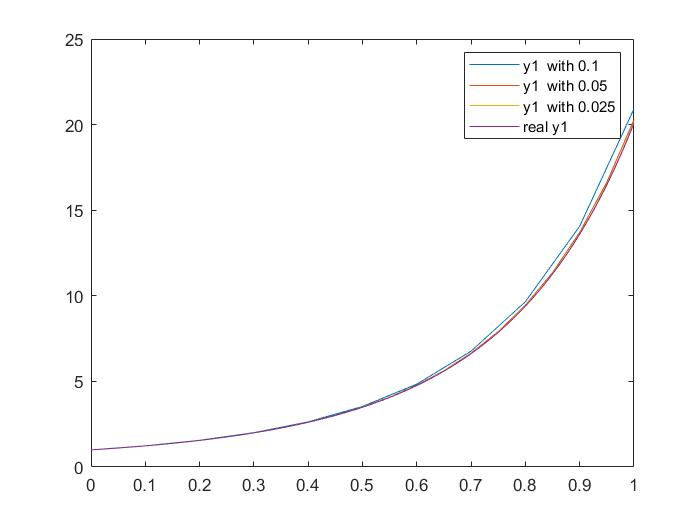
\includegraphics[width=9cm]{y1_trap.jpg} 
 \end{center}
 
 and for y2, we can hardly see the difference of the plots, so I zoom in to get the second graph:
 \begin{center}
  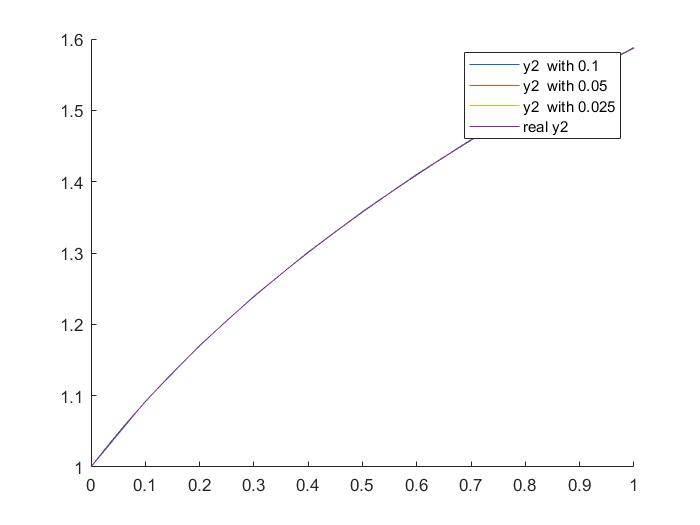
\includegraphics[width=7cm]{y2_trap.jpg} 
   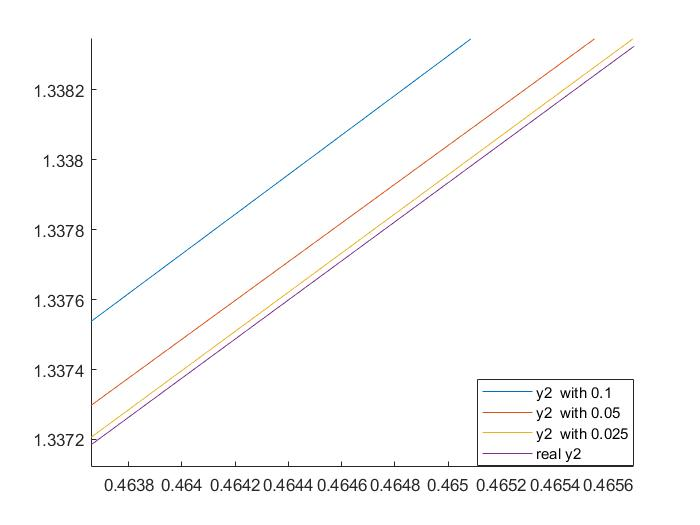
\includegraphics[width=7cm]{y2_trap_zoom.jpg} 
 \end{center}
 
 and the error at $t=1$ for different h is:
  \begin{center}
  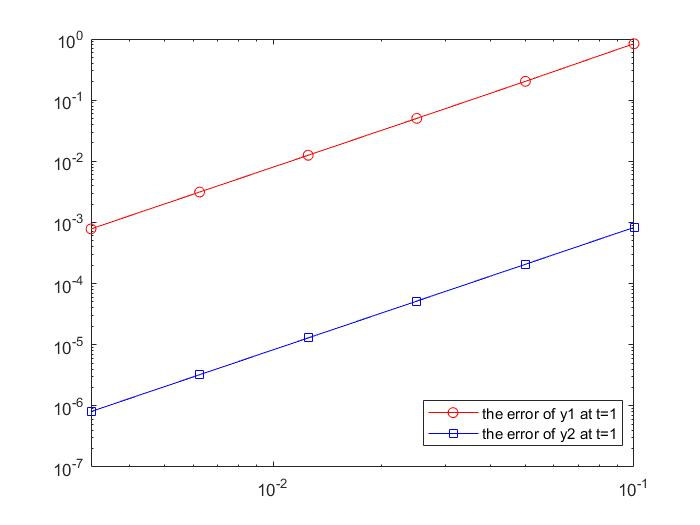
\includegraphics[width=7cm]{trap_loglog.jpg}  
 \end{center}
 \item
 We can observe that Trapezoidal method have a higher accuracy than the forward Euler method, and have a higher order of error term, to see this clearly, we can plot two error loglog graph onto the same picture:
 \begin{center}
  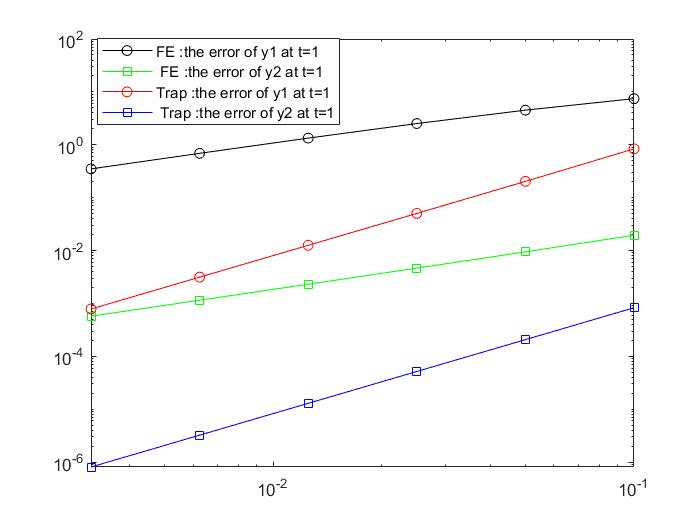
\includegraphics[width=7cm]{combine_loglog.jpg}  
 \end{center}
 
 Obviously, the slope of Trapezoidal method is steeper than that of forward Euler method, which means Trapezoidal method will converge faster than forward Euler Method as $h$ decrease. To be more specifically, forward Euler generate an error of order 1, and Trapezoidal method generate an error of order 2, and this conclusion consists of the graph we draw earlier that we can directly distinguish the lines and see the convergence of forward Euler method, but for Trapezoid method,  we can hardly see the differences of the graph directly. And we can compute the slope of two method, four plotted lines, which are  approximately -1 and -2, in the sense of first and second order error
 \begin{small}
 \lstinputlisting[language=Matlab,caption={slope}]{slope.txt}
 \end{small}
 
 
 
 Besides that, we can observe that $y2$ (the second function) always generate smaller error than $y1$ (the first function) during the approximation process, and when we observe the figures, we can find that the graph of $y2$ is smoother than that of $y1$ in the interval $[0,1]$, this make sense that we can always approximate the function with smaller local change better than the function with local change dramatically.
\end{enumerate}
\item
\begin{itemize}
\item \textbf{Forward Euler Method}:\\
\begin{align*}
x_{j+1}&= x_j+ h \cdot f_x(\phi_j, x(\phi_j),y(\phi_j))\\
&=x_j - h \cdot y(\phi_j)\\
&= x_j - h \cdot y_j\\
y_{j+1}&= y_j+ h \cdot f_y(\phi_j, x(\phi_j),y(\phi_j))\\
&=y_j + h \cdot x(\phi_j)\\
&= y_j + h \cdot x_j
\end{align*}
\item \textbf{Backward Euler Method}:\\
\begin{align*}
x_{j+1}&= x_j+ h \cdot f_x(\phi_{j+1}, x(\phi_{j+1}),y(\phi_{j+1}))\\
&=x_j - h \cdot y(\phi_{j+1})\\
&= x_j - h \cdot y_{j+1}\\
y_{j+1}&= y_j+ h \cdot f_y(\phi_{j+1}, x(\phi_{j+1}),y(\phi_{j+1}))\\
&=y_j+ h \cdot x(\phi_{j+1})\\
&= y_j+ h \cdot x_{j+1}\\
x_{j+1}&= x_j - h \cdot y_j- h^2 \cdot x_{j+1}\\
&=\dfrac{x_j - h \cdot y_j}{1+h^2}
\end{align*}
\item \textbf{Trapezoidal Method}:\\

\begin{align*}
x_{j+1}&= x_j+ \frac{h}{2} \left(f_x(\phi_j, x(\phi_j),y(\phi_j))+ f_x(\phi_{j+1}, x(\phi_{j+1}),y(\phi_{j+1}))\right)\\
&=x_j - \frac{h}{2} \left(y(\phi_{j})+ y(\phi_{j+1})\right)\\
&=x_j - \frac{h}{2} \left(y_{j}+ y_{j+1}\right)\\
y_{j+1}&= y_j+ \frac{2}{h} \left(f_y(\phi_j, x(\phi_j),y(\phi_j))+ f_y(\phi_{j+1}, x(\phi_{j+1}),y(\phi_{j+1}))\right)\\
&=y_j+\frac{h}{2} \left(x(\phi_{j})+ x(\phi_{j+1})\right)\\
&=y_j+\frac{h}{2} \left(x_{j}+ x_{j+1}\right)\\
x_{j+1}&= x_j - \frac{h}{2} \left(y_{j}+ y_{j+1}\right)\\
&= x_j - \frac{h}{2} \left(y_{j}+ y_j+\frac{h}{2} \left(x_{j}+ x_{j+1}\right)\right)\\
&=x_j - h \cdot y_j-\frac{h^2}{4}\left(x_{j}+ x_{j+1}\right)
\end{align*}\begin{align*}
\left(1+\frac{h^2}{4}\right)x_{j+1}&=\left(1-\frac{h^2}{4}\right)x_{j} - h \cdot y_j\\
\therefore x_{j+1}&=\dfrac{\left(1-\frac{h^2}{4}\right)x_{j} - h \cdot y_j}{1+\frac{h^2}{4}}
\end{align*}
\end{itemize}


And the code is: 
 \lstinputlisting[language=Matlab, numbers=left, stepnumber=1, firstline=1, frame = single,caption={circle.m}]{circle.m}
 
 with the graph of Forward Euler, Backward Euler and  Trapezoidal Method:
  \begin{center}
  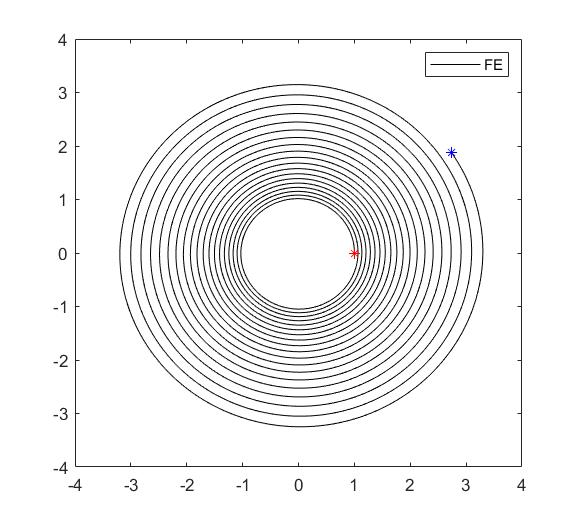
\includegraphics[width=5cm]{circle_FE.jpg}  
  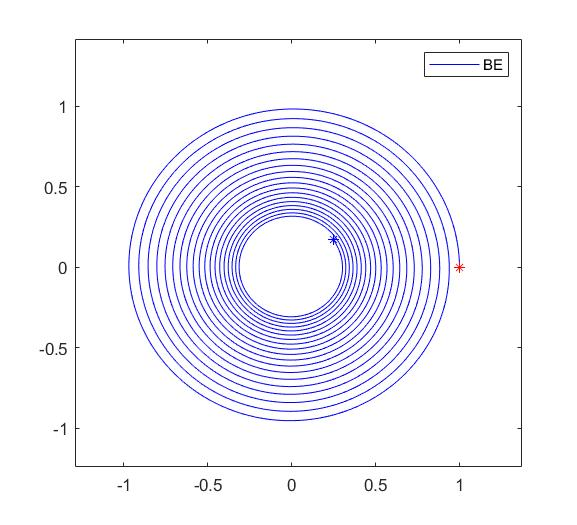
\includegraphics[width=5cm]{circle_BE.jpg}  
  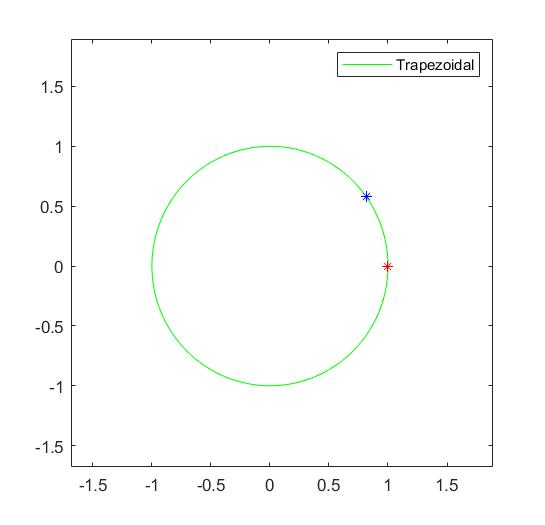
\includegraphics[width=5cm]{circle_trap.jpg} 
 \end{center}
 And since I make the red point to be the beginning, and the blue one to be the ending, so we can see that FE spirals out, BE spirals in, and Trapezoidal method gives us the circle we desired.
 
 
 For Forward Euler Method, we can examine that\begin{align*}
 x_{j+1}^2+y_{j+1}^2&=(x_j-h\cdot y_j)^2+ (y_j+hx_j)^2\\
 &=x_j^2-2hx_jy_j+h^2y_j^2+y_j^2+2hx_jy_j+h^2x_j^2\\
 &=x_j^2+h^2y_j^2+y_j^2+h^2x_j^2\\
 &=(1+h^2)(x_j^2+y_j^2)\\
 &> x_j^2+y_j^2
 \end{align*}
 Therefore, the radius increase in each step, so it spirals out.
 
 For Backward Euler Method, we can examine that \begin{align*}
  x_{j+1}^2+y_{j+1}^2&=x_{j+1}^2+(y_j+h\cdot x_{j+1})^2\\
 &= x_{j+1}^2+y_j^2+2h x_{j+1}y_j+h^2x_{j+1}^2\\
 &=(1+h^2) x_{j+1}^2+y_j^2+2h x_{j+1}y_j\\
  &=\dfrac{(1+h^2)(x_j-hy_j)^2}{(1+h^2)^2}+y_j^2+\dfrac{2hy_j(x_j-hy_j)}{1+h^2}\\
   &=\dfrac{(1+h^2)(x_j-hy_j)^2}{(1+h^2)^2}+y_j^2+\dfrac{2hy_j(x_j-hy_j)}{1+h^2}\\
 &=\dfrac{(x_j-hy_j)^2+2hy_j(x_j-hy_j)}{1+h^2}+y_j^2\\
         \end{align*}\begin{align*}
  &=\dfrac{x_j^2-2hx_jy_j+h^2y_j^2+2hx_jy_j-2h^2y_j^2}{1+h^2}+y_j^2\\
    &=\dfrac{x_j^2-h^2y_j^2}{1+h^2}+y_j^2\\
    &=x_j^2+y_j^2+\dfrac{-h^2x_j^2-h^2y_j^2}{1+h^2}\\
    & < x_j^2+y_j^2
 \end{align*}
  Therefore, the radius decrease in each step, so it spirals in.
  
  For Trapezoidal method, we can examine that \begin{align*}
  x_{j+1}^2+y_{j+1}^2&= x_{j+1}^2+\left( y_j+\dfrac{h}{2}(x_j+x_{j+1})\right)^2\\
  &= x_{j+1}^2+\left( y_j+\dfrac{h}{2}\dfrac{(1+\frac{h^2}{4}+1-\frac{h^2}{4})x_j-hy_j}{1+\frac{h^2}{4}}\right)^2\\
    &= x_{j+1}^2+\left( y_j+\dfrac{h}{2}\dfrac{2x_j-hy_j}{1+\frac{h^2}{4}}\right)^2\\
        &= x_{j+1}^2+\left(\dfrac{hx_j}{1+\frac{h^2}{4}}+\dfrac{(2-\frac{h^2}{2})y_j}{2+\frac{h^2}{2}}\right)^2\\
   &= x_{j+1}^2+\left(\dfrac{2hx_j+(2-\frac{h^2}{2})y_j}{2+\frac{h^2}{2}}\right)^2\\
    &= \dfrac{(1-\frac{h^2}{4})^2 -2hx_jy_j(1-\frac{h^2}{4})+h^2y_j^2}{(1+\frac{h^2}{4})^2}+\left(\dfrac{2hx_j+(2-\frac{h^2}{2})y_j}{2+\frac{h^2}{2}}\right)^2\\
      &= \dfrac{(1-\frac{h^2}{4})^2x_j^2 -2hx_jy_j(1-\frac{h^2}{4})+h^2y_j^2}{(1+\frac{h^2}{4})^2}+\left(\dfrac{hx_j+(1-\frac{h^2}{4})y_j}{1+\frac{h^2}{4}}\right)^2\\
            &= \dfrac{(1-\frac{h^2}{4})^2x_j^2 -2hx_jy_j(1-\frac{h^2}{4})+h^2y_j^2+h^2x_j^2+2hx_jy_j(1-\frac{h^2}{4})+(1-\frac{h^2}{4})^2y_j^2}{(1+\frac{h^2}{4})^2}\\
    &= \dfrac{(1-\frac{h^2}{4})^2x_j^2 +h^2y_j^2+h^2x_j^2+(1-\frac{h^2}{4})^2y_j^2}{(1+\frac{h^2}{4})^2}\\
    &= \dfrac{(1-\frac{h^2}{2}+\frac{h^4}{16})x_j^2 +h^2y_j^2+h^2x_j^2+(1-\frac{h^2}{2}+\frac{h^4}{16})y_j^2}{(1+\frac{h^2}{2}+\frac{h^4}{16})}\\
       &= \dfrac{(1+\frac{h^2}{2}+\frac{h^4}{16})x_j^2 +(1+\frac{h^2}{2}+\frac{h^4}{16})y_j^2}{(1+\frac{h^2}{2}+\frac{h^4}{16})}\\
       &=x_j^2+y_j^2
  \end{align*}
    Therefore, the radius does not change, so it's a circle we deserved.
  
  \item
  For four-point Gaussian, we can firstly derive the Legendre Polynomial of degree 4, which is \begin{align*}
  P_2(x) &=\dfrac{1}{2}(3x^2-1)\\
  P_3(x) &=\dfrac{1}{2}(5x^3-3x)\\
  4P_4(x) &= 7xP_3(x)-3P_2(x)\\
  &=\dfrac{7}{2}(5x^4-3x^2)-\dfrac{3}{2}(3x^2-1)\\
  &=\dfrac{35x^4}{2}-\dfrac{30x^2}{2}+\dfrac{3}{2}\\
  P_4(x)&=\dfrac{35x^4}{8}-\dfrac{15x^2}{4}+\dfrac{3}{8}\\
\end{align*}
And we can solve $P_4(x) =0$  to get the nodes:\begin{align*}
\dfrac{35x^4}{8}-\dfrac{15x^2}{4}+\dfrac{3}{8}&=0\\
35x^4-30x^2+3&=0\\
x^2&=\dfrac{30\pm \sqrt{900-4\cdot 35\cdot 3}}{70}\\
&=\dfrac{30\pm \sqrt{480}}{70}\\
&=\dfrac{15\pm 2\sqrt{30}}{35}\\
x&=\pm \sqrt{\dfrac{15\pm 2\sqrt{30}}{35}}\\
x_1 &= -\sqrt{\dfrac{15+ 2\sqrt{30}}{35}}\\
x_2&=-\sqrt{\dfrac{15- 2\sqrt{30}}{35}}\\
x_3 &= \sqrt{\dfrac{15- 2\sqrt{30}}{35}}\\
x_4&=\sqrt{\dfrac{15+ 2\sqrt{30}}{35}}
\end{align*}

For the weight, since \begin{align*}
\int_{-1}^1 f(x) dx &\approx \int_{-1}^1 Q(x) dx\\
&=\int_{-1}^1 \sum_{j=1}^{n+1} L_j(x) f(x_j) dx\\
&=\int_{-1}^1 \sum_{j=1}^{4} L_j(x)dx f(x_j)\\
\end{align*}
Based on four points, \begin{align*}
L_1(x) &= \dfrac{(x-x_2)(x-x_3)(x-x_4)}{(x_1-x_2)(x_1-x_3)(x_1-x_4)}\\
L_2(x) &= \dfrac{(x-x_1)(x-x_3)(x-x_4)}{(x_2-x_1)(x_2-x_3)(x_2-x_4)}\\
L_3(x) &= \dfrac{(x-x_1)(x-x_2)(x-x_4)}{(x_3-x_1)(x_3-x_2)(x_3-x_4)}\\
L_4(x) &= \dfrac{(x-x_1)(x-x_2)(x-x_3)}{(x_4-x_1)(x_4-x_2)(x_4-x_3)}
\end{align*}
And we can get \begin{align*}
\omega_1&=\int_{-1}^1L_1(x) dx\\
&=\int_{-1}^1 \dfrac{(x-x_2)(x-x_3)(x-x_4)}{(x_1-x_2)(x_1-x_3)(x_1-x_4)} dx\\
&=\dfrac{1}{(x_1-x_2)(x_1-x_3)(x_1-x_4)}\int_{-1}^1(x-x_2)(x-x_3)(x-x_4) dx\\
&=\dfrac{1}{(x_1-x_2)(x_1-x_3)(x_1-x_4)}\int_{-1}^1x^3-(x_2+x_3+x_4)x^2+(x_2x_3+x_2x_4+x_3x_4)x - x_2x_3x_4 dx\\
&=-\dfrac{2}{3}\dfrac{3x_2x_3x_4+x_2+x_3+x_4}{(x_1-x_2)(x_1-x_3)(x_1-x_4)}
        \end{align*}\begin{align*}
\omega_2&=\int_{-1}^1L_2(x) dx\\
&=-\dfrac{2}{3}\dfrac{3x_1x_3x_4+x_1+x_3+x_4}{(x_2-x_1)(x_2-x_3)(x_2-x_4)}\\
\omega_3&=\int_{-1}^1L_3(x) dx\\
&=-\dfrac{2}{3}\dfrac{3x_1x_2x_4+x_1+x_2+x_4}{(x_3-x_1)(x_3-x_2)(x_3-x_4)}\\
\omega_4&=\int_{-1}^1L_4(x) dx\\
&=-\dfrac{2}{3}\dfrac{3x_1x_2x_3+x_1+x_2+x_3}{(x_4-x_1)(x_4-x_2)(x_4-x_3)}
\end{align*}

Since \begin{align*}
x_1 - x_2 &= \sqrt{\dfrac{15- 2\sqrt{30}}{35}} - \sqrt{\dfrac{15+2\sqrt{30}}{35}}\\
x_1-x_3&=-\sqrt{\dfrac{15+ 2\sqrt{30}}{35}}-\sqrt{\dfrac{15- 2\sqrt{30}}{35}}\\
x_1-x_4&=-2\sqrt{\dfrac{15+ 2\sqrt{30}}{35}}\\
x_2-x_3&=-2\sqrt{\dfrac{15- 2\sqrt{30}}{35}}\\
x_2-x_4&=-\sqrt{\dfrac{15- 2\sqrt{30}}{35}}-\sqrt{\dfrac{15+ 2\sqrt{30}}{35}}\\
x_3-x_4 &=\sqrt{\dfrac{15- 2\sqrt{30}}{35}}-\sqrt{\dfrac{15+ 2\sqrt{30}}{35}}
\end{align*}
Therefore
\begin{align*}
\omega_1&=-\dfrac{2}{3}\dfrac{-3\cdot \dfrac{15-2\sqrt{30}}{35}\sqrt{\dfrac{15+2\sqrt{30}}{35}}+\sqrt{\dfrac{15+2\sqrt{30}}{35}}}{(x_1-x_2)(x_1-x_3)(x_1-x_4)}\\
&=\dfrac{2}{3}\dfrac{-3\cdot \dfrac{15-2\sqrt{30}}{35}\sqrt{\dfrac{15+2\sqrt{30}}{35}}+\sqrt{\dfrac{15+2\sqrt{30}}{35}}}{2(\dfrac{15+2\sqrt{30}}{35} -\dfrac{15- 2\sqrt{30}}{35} )\sqrt{\dfrac{15+ 2\sqrt{30}}{35}}}
        \end{align*}\begin{align*}
&=\dfrac{- \dfrac{15-2\sqrt{30}}{35}\sqrt{\dfrac{15+2\sqrt{30}}{35}}+\sqrt{\dfrac{15+2\sqrt{30}}{315}}}{(\dfrac{4\sqrt{30}}{35} )\sqrt{\dfrac{15+ 2\sqrt{30}}{35}}}\\
&=\dfrac{- \dfrac{15-2\sqrt{30}}{35}+\frac{1}{3}}{(\dfrac{4\sqrt{30}}{35} )}\\
&=\dfrac{- 15+2\sqrt{30}+\frac{35}{3}}{4\sqrt{30}}\\
&=-\dfrac{\sqrt{30}}{36}+\dfrac{1}{2}
\end{align*}
\begin{align*}
\omega_2&=-\dfrac{2}{3}\dfrac{-3\cdot \dfrac{15+2\sqrt{30}}{35}\sqrt{\dfrac{15-2\sqrt{30}}{35}}+\sqrt{\dfrac{15-2\sqrt{30}}{35}}}{(x_2-x_1)(x_2-x_3)(x_2-x_4)}\\
&=\dfrac{2}{3}\dfrac{-3\cdot \dfrac{15+2\sqrt{30}}{35}\sqrt{\dfrac{15-2\sqrt{30}}{35}}+\sqrt{\dfrac{15-2\sqrt{30}}{35}}}{2(\dfrac{15-2\sqrt{30}}{35} -\dfrac{15+ 2\sqrt{30}}{35} )\sqrt{\dfrac{15- 2\sqrt{30}}{35}}}\\
&=\dfrac{2}{3}\dfrac{-3\cdot \dfrac{15+2\sqrt{30}}{35}+1}{2(\dfrac{15-2\sqrt{30}}{35} -\dfrac{15+ 2\sqrt{30}}{35} )}\\
&=-\dfrac{- (15+2\sqrt{30})+\frac{35}{3}}{4\sqrt{30}}\\
&=\dfrac{\sqrt{30}}{36}+\dfrac{1}{2}
\end{align*}
\begin{align*}
\omega_3&=-\dfrac{2}{3}\dfrac{-3\cdot \dfrac{15+2\sqrt{30}}{35}\sqrt{\dfrac{15-2\sqrt{30}}{35}}+\sqrt{\dfrac{15-2\sqrt{30}}{35}}}{(x_3-x_1)(x_3-x_2)(x_3-x_4)}\\
&=\dfrac{2}{3}\dfrac{-3\cdot \dfrac{15+2\sqrt{30}}{35}\sqrt{\dfrac{15-2\sqrt{30}}{35}}+\sqrt{\dfrac{15-2\sqrt{30}}{35}}}{2(\dfrac{15-2\sqrt{30}}{35} -\dfrac{15+ 2\sqrt{30}}{35} )\sqrt{\dfrac{15- 2\sqrt{30}}{35}}}\\
&=\dfrac{\sqrt{30}}{36}+\dfrac{1}{2}
\end{align*}
\begin{align*}
\omega_4&=-\dfrac{2}{3}\dfrac{-3\cdot \dfrac{15-2\sqrt{30}}{35}\sqrt{\dfrac{15+2\sqrt{30}}{35}}+\sqrt{\dfrac{15+2\sqrt{30}}{35}}}{(x_4-x_1)(x_4-x_2)(x_4-x_3)}\\
&=\dfrac{2}{3}\dfrac{-3\cdot \dfrac{15-2\sqrt{30}}{35}\sqrt{\dfrac{15+2\sqrt{30}}{35}}+\sqrt{\dfrac{15+2\sqrt{30}}{35}}}{2(\dfrac{15+2\sqrt{30}}{35} -\dfrac{15- 2\sqrt{30}}{35} )\sqrt{\dfrac{15+ 2\sqrt{30}}{35}}}\\
&=-\dfrac{\sqrt{30}}{36}+\dfrac{1}{2}\\
\end{align*}
 \end{enumerate}
 
 \section*{Appendix}
 
 
 Code for Question 3f:
  \lstinputlisting[language=Matlab, numbers=left, stepnumber=1, firstline=1, frame = single,caption={Trap.m}]{Trap.m}
  
    \lstinputlisting[language=Matlab, numbers=left, stepnumber=1, firstline=1, frame = single,caption={trap2\_graph.m}]{trap2_graph.m}
    
       \lstinputlisting[language=Matlab, numbers=left, stepnumber=1, firstline=1, frame = single,caption={trap\_loglog.m}]{trap_loglog.m}
\end{document}